%% SIGCOMM 2027 format (acmart, sigconf), with author names: a course report, not a blind submission.
%% Template: https://github.com/epfl-laser/sigcomm27-latex-template (acmart.cls and the .bst are copied from it).
%% Body text is the same as ../paper.tex; edit both, or retire ../paper.tex once this one is the report.
%% Build: make   (or latexmk -pdf paper; on Overleaf, set TeX Live 2025 or later)
\documentclass[sigconf]{acmart}

\usepackage{booktabs}
\usepackage{xcolor}
\usepackage{balance}

% Marks a number that waits for an experiment. Must not appear in the submitted PDF.
\newcommand{\pending}[1]{\textcolor{red}{[#1]}}

% No ACM copyright block, reference format or CCS concepts: this is a course report.
\setcopyright{none}
\renewcommand\footnotetextcopyrightpermission[1]{}
\settopmatter{printacmref=false, printccs=false, printfolios=true}
\acmConference[CS G525]{CS G525 Advanced Computer Networks, Project Report}{November 2026}{BITS Pilani, India}

% Lets TeX stretch spaces a little more instead of pushing words into the margin.
\setlength{\emergencystretch}{1.5em}

\begin{document}

\title{Ask Less, Tell More: Rule Granularity, Not Prediction, Explains the Gains of OpenFlow Rule Pre-Installation}

% Four authors on one line, one shared affiliation. (Separate \author commands make acmart
% stack the names in a column.) \shortauthors below sets the running head.
\author{Dhaduk Mrudul, Nisarg Vagh, Prachit Deshinge, Mukul Saini}
\affiliation{\institution{Department of Computer Science and Information Systems, BITS Pilani}\country{India}}
\renewcommand{\shortauthors}{Dhaduk, Vagh, Deshinge and Saini}

\begin{abstract}
A reactive OpenFlow controller makes each new flow's first packet wait for a rule; a proactive one pre-installs a rule for every host pair. Alternatives, from rule caches to learned predictors, beat plain reactive installation but are rarely compared with reactive installation using equally coarse rules. We test them on emulated networks (Mininet, Open vSwitch, POX): a campus tree, a fat-tree and the Abilene backbone, giving every controller identical flows. Reactive destination rules, with no prediction, find a rule for 93.6--99.6\% of new connections at 11--16 hosts, come within 0.3\,ms of proactive's small-flow median on the campus tree and Abilene, and beat a popularity-based hybrid and its hindsight oracle in hit rate in every seed on three networks. A trace-replay model matching all 46 measured coarse-rule runs within 0.1 points extends this to 1,024 hosts: prediction pays only where flows per host pair are few and popularity is skewed. A destination-rule controller receiving copies of TCP SYN, FIN and RST packets stays within 0.9\,ms of proactive on three of four networks and hears of all 46,641 connections. A 50\,ms one-way control-channel delay adds over a second to exact-match reactive's small-flow median and under 0.9\,ms to tap's, proactive's and destination rules'.
\end{abstract}

\keywords{software-defined networking, OpenFlow, flow-rule installation, benchmarking, rule caching, prediction}

\maketitle

\section{Introduction}

An OpenFlow switch forwards a packet only if it matches a rule. A \emph{reactive} controller installs a rule when a flow's first packet reaches it as a PACKET\_IN; a \emph{proactive} controller installs rules before traffic arrives. Reactive installation keeps tables small and gives the controller per-flow control, at the cost of a setup delay on every new flow and a controller request per flow per switch~\cite{ethane,difane,devoflow}. Proactive installation removes both costs but needs a rule for every host pair.

A large body of work sits between the two: adaptive timeouts~\cite{smarttime,ahihta}, caches of popular rules~\cite{cacheflow}, proactive/reactive hybrids~\cite{pard,kim2022}, and predictors, increasingly machine-learned, that install rules before the flows that need them~\cite{batista2024,rouf2025}. Each was shown to beat a reactive baseline. Where the proposed strategy installs coarser rules than that baseline, the comparison changes two things at once: \emph{when} a rule is installed, and \emph{how coarse} it is. The common reactive baseline, the learning switch of NOX and POX, installs an exact-match rule for each transport connection. Such a rule is almost never reused, because every new TCP connection has a new source port. A pre-installed rule that matches a host pair, in contrast, serves every later connection of that pair. A predictor compared with exact-match reactive therefore gets credit for coarseness as well as for prediction.

We ask how much of the gain remains when the baseline uses the same coarse rules, and where prediction has room at all. Our contributions:
\begin{enumerate}
\item \textbf{A benchmark} of rule-installation strategies along four axes (timing, granularity, path choice, selection of pre-installed pairs) with identical flow schedules for every controller, four workloads taken from published measurements and real traffic matrices, three network types, and two reference points for pre-installing a fixed set of pairs: a random set (a floor) and the run's busiest pairs chosen in hindsight (an oracle). With an exact-match fallback the oracle is the best fixed set; it is not a bound for a predictor that changes its set over time, nor, with a coarse-rule fallback, for a fixed one (Sections~\ref{sec:design} and~\ref{sec:scale}).
\item \textbf{The granularity finding.} Reactive with pair or destination rules finds a rule for 86--100\% of new connections at 11--16 hosts with no prediction, and has a higher hit rate than a budgeted popularity hybrid and its static oracle in every seed of three networks (Section~\ref{sec:granularity}). Long timeouts give almost no benefit for short-flow traffic.
\item \textbf{A validated scale model and the regime map.} A trace replay reproduces the hit rate of the 46 measured wildcard runs (mean absolute error at most 0.1 points); on fat-trees of up to 1,024 hosts it shows that whether prediction pays depends on pair-popularity skew as well as size: at Zipf 1 only where flows per host pair fall to 2--3 (54 hosts at 5\% load, about 432 at 30\% load), at Zipf 0 and 0.5 never, and at Zipf 1.5 by a few points at almost every size (Section~\ref{sec:scale}).
\item \textbf{Asking versus telling.} A controller that forwards on destination rules and receives copies of TCP SYN, FIN and RST packets keeps proactive's speed and reactive's per-connection visibility (Section~\ref{sec:tap}).
\end{enumerate}
Of the 11 pre-installation papers in our survey (Section~\ref{sec:related}), none compares a predictor that pre-installs coarser rules with a reactive baseline using the same coarse rules, and only one reports an upper bound, in the material available to us (the full text of seven, the abstract of four). All code, flow schedules and per-flow results are released.\footnote{\url{https://github.com/PrachitDeshinge-324/Openflow_SDN}.}

\section{Background and related work}\label{sec:related}

\textbf{Setup cost.} Ethane~\cite{ethane} and DIFANE~\cite{difane} measured the delay of reactive setup; DevoFlow~\cite{devoflow} showed that per-flow control overloads switch control paths and argued for wildcard rules by default, giving up visibility of most flows. Controller benchmarks~\cite{tootoonchian} measure peak request rates under synthetic load. We measure setup cost under realistic traffic, and show that the choice DevoFlow made for scalability also removes most of the case for prediction.

\textbf{Caching, timeouts and hybrids.} CacheFlow~\cite{cacheflow} caches popular rules and reports high hit rates on Zipf traffic. SmartTime~\cite{smarttime} and AH-IHTA~\cite{ahihta} tune timeouts. PARD~\cite{pard} forwards on coarse proactive rules while the controller installs detailed rules in the background; Kim et al.~\cite{kim2022} choose per flow between proactive and reactive in simulation. None compares against the others, or against a coarse-rule reactive controller, on the same traffic.

\textbf{Prediction.} Our survey covers 11 papers that pre-install rules using a predictor and 14 that use learning or heuristics for eviction and timeouts. Of the 11, three compare only against plain reactive installation (e.g., an LSTM scheduler on POX that reports 51\% lower response time~\cite{batista2024}), four against reactive installation and other published schemes~\cite{kim2022}, one against its own earlier variants, two do not name their baseline in the abstract available to us, and one, a study of preloading predicted flows into a virtual switch's cache, compares no prediction with perfect prediction; 8 of the 9 that state their traffic use periodic IoT or mobility traffic. We read seven of the 11 in full and four from the abstract only. In two of the seven, the pre-installed rule is the one the reactive baseline installs, so coarseness plays no part: the gain comes from installing the rule before a 1\,s idle timeout, shorter than the traffic's period, lets it expire, and no baseline with a longer timeout is reported. In one, pre-installed rules match a traffic class while reactive rules match a host pair, and no reactive baseline with class rules is reported. None of the seven compares coarser pre-installed rules with a reactive baseline of the same granularity, and only the virtual-switch study reports an upper bound (its perfect-prediction case); for the four abstract-only papers we can say only that the abstract mentions neither. We also know of one pre-installation paper outside the survey, a reinforcement-learning scheme that installs rules for flows not yet seen~\cite{hariri2024}; we could not access it and do not count it. Where a simple baseline is reported in the eviction literature, the learned method's margin is small: a DQN eviction policy closes about 8\% of LFU's gap to the optimal eviction policy, which is about one point of hit rate~\cite{rouf2025}. Analytical models of reactive signalling and table occupancy exist~\cite{metter2017}; we use the same idea of replaying arrivals through a timeout cache, and validate it against measurement.

\textbf{Monitoring.} Flow records (sFlow, IPFIX~\cite{ipfix}) report flows after the fact or by sampling. Everflow~\cite{everflow} matches TCP SYN, FIN and RST packets in data-centre switches and mirrors them to collectors for tracing; FlowSense~\cite{flowsense} infers utilisation from the controller's existing messages. Our tap controller (Section~\ref{sec:tap}) uses Everflow's match inside the OpenFlow control loop, so the copy reaches the controller as a PACKET\_IN when the connection starts. We do not claim the mechanism as new; we measure what it changes in the reactive/proactive trade-off.

\textbf{Paths.} Fat-trees need ECMP or flow scheduling to use their capacity~\cite{alfares,hedera}. These works do not consider how rules are installed; we measure both together.

\section{Benchmark design}\label{sec:design}

\textbf{Testbed.} Mininet 2.3.0~\cite{mininet}, Open vSwitch 3.7.1~\cite{ovs} with the kernel datapath, POX 0.7.0 and OpenFlow 1.0, on one laptop (Windows 11 with WSL2, x86\_64, 16 hardware threads; every testbed number in this paper except the LSTM batch of Section~\ref{sec:granularity} comes from it, with WSL2 kernel 6.18.33 for the October batches of Table~\ref{tab:granularity} and 6.18.58 for the November batches of Tables~\ref{tab:tap} and~\ref{tab:delay}). The controller runs on the same machine. The repository's \texttt{docs/Reproduce.md} gives, for each table and figure, the command, the result folders and the machine. ARP tables are static and IPv6 is disabled, so neither reaches the controller.

\textbf{Controllers.} Table~\ref{tab:controllers} lists the strategies. All topology-aware controllers share one implementation that exposes the four axes as options, so two controllers differ only in the axis being compared.

\begin{table}[t]
\caption{Controllers. Timeouts: idle 10\,s, hard 30\,s unless stated.}\label{tab:controllers}
\centering\footnotesize
\begin{tabular}{@{}p{2.3cm}p{5.6cm}@{}}
\toprule
Name & Behaviour \\
\midrule
Reactive (tree) & POX learning switch, exact-match rule per connection per switch, over a spanning tree \\
Reactive, long & the same, idle 60\,s / hard 300\,s \\
Reactive, exact & exact-match rules on shortest paths (topology known) \\
Reactive, pair & one rule per (source, destination) MAC pair on the first miss \\
Reactive, dest. & one rule per destination MAC on the first miss \\
Counter $B$\% & reactive exact, plus pair rules for the top $B$\% of pairs by a decaying activity score (decay 0.97/s, hysteresis 1.5) \\
Oracle $B$\% & pair rules for the $B$\% of pairs that carry the most flows in this run, installed before the first flow. With this exact-match fallback, the best \emph{fixed} set in hindsight; not a bound for a predictor that changes its set \\
Random $B$\% & pair rules for $B$\% random pairs, before the first flow \\
LSTM $B$\% & as Counter, but pairs ranked by a small LSTM's forecast of next-second activity (Section~\ref{sec:granularity}) \\
Proactive & one rule per host pair on its lowest-delay path (ECMP on fat-trees, hashed per pair) \\
Tap & destination rules for every host, plus 3 rules per host that copy TCP SYN, FIN, RST to the controller \\
\bottomrule
\end{tabular}
\end{table}

\textbf{Networks.} A two-level campus tree (16 hosts, 5 switches, 240 ordered pairs); a $k{=}4$ fat-tree (16 hosts, 20 switches) and a $k{=}6$ fat-tree (54 hosts, 45 switches, 2,862 pairs); and the Abilene backbone (11 cities, 14 links, the real 2.48\,Gbit/s Atlanta--Indianapolis link scaled accordingly, one-way delays of 1.33--11.03\,ms from fibre distance). Links run at 100\,Mbit/s.

\textbf{Workloads.} \emph{University}: flow sizes from Benson et al.'s university data centres~\cite{benson}, Weibull gaps per edge switch with 80\% between 4 and 40\,ms. \emph{Web search} and \emph{data mining}: the DCTCP~\cite{dctcp} and VL2~\cite{vl2} size distributions as used by pFabric~\cite{pfabric} and PIAS~\cite{pias}, Poisson arrivals at 30\% load (5\% at $k{=}6$). \emph{ISP}: one day of real Abilene traffic matrices~\cite{zhang2005} replayed in 30\,s, SURGE flow sizes~\cite{surge}. Host-pair popularity is Zipf with exponent 1, as assumed by CacheFlow~\cite{cacheflow}, with a uniform control; the ISP workload uses the real matrices. Each flow is a TCP connection that sends its bytes and waits for a one-byte reply.

\textbf{Fairness and statistics.} The flow schedule is computed from a seed before the run, so every controller receives exactly the same flows. All controllers of a scenario run for each seed in one batch. Tables give the mean of 5 seeds (3 at $k{=}6$) with the half-width of the 95\% confidence interval (Student's $t$). Because a seed fixes the flows, two controllers are compared \emph{per seed}: we report the mean of the $n$ per-seed differences with its 95\% interval (Student's $t$, $n{-}1$ degrees of freedom; $t{=}2.78$ for $n{=}5$, $4.30$ for $n{=}3$), and call a difference resolved only when the interval excludes zero. An interval containing zero bounds the difference; it does not show that two controllers are equal, and we make no equivalence claim, since no equivalence margin was fixed before the runs. Absolute times are compared only within one batch (one table): batches on different days give different times for the same controller (proactive's small-flow median on the campus tree is 1.49\,ms in Table~\ref{tab:granularity} and 0.94\,ms in Table~\ref{tab:tap}).

\textbf{Metrics.} \emph{Hit rate}: share of new TCP connections whose SYN finds a rule at the sender's switch, counted by the controller. It is defined for controllers that react to misses; proactive and tap install every forwarding rule before traffic starts, so their hit rate is 100\% by construction and is not listed. \emph{Small-flow FCT}: median completion time of flows under 100\,KB. Controller load: PACKET\_IN/s and controller CPU. \emph{Rules}: peak rules over all switches, read from the switches. \emph{Visibility}: share of connections the controller learns of.

\section{Results on the testbed}\label{sec:granularity}

\subsection{Exact-match reactive pays twice}
Under realistic traffic, exact-match reactive sends 10.5--12.9 PACKET\_INs per flow and its small flows are 2.2--28$\times$ slower than proactive's. On networks with loops part of this is path, not setup: the spanning tree switches off 4 of Abilene's 14 links, so 70\% of pairs take a longer path (mean delay stretch 1.58, up to 4.47). Running the same exact-match controller on shortest paths splits the small-flow median penalty on Abilene into about 41\,ms of path and 10\,ms of setup. Long timeouts (60\,s/300\,s) made no flows faster in any of four scenarios (paired small-flow median $+0.5$ to $+2.0$\,ms, resolved only with uniform pairs: $+2.0$ [$+1.9$, $+2.2$]\,ms) and cut controller requests by at most 4\% (resolved only on the campus tree: $-99$ [$-112$, $-86$] and $-70$ [$-94$, $-45$] PACKET\_IN/s with Zipf and uniform pairs), with 2.2--3.0$\times$ the rules: an exact-match rule is almost never reused by a new connection however long it lives.

\subsection{Granularity explains the hybrid's gain}\label{sec:hybrid}

\begin{table}[t]
\caption{Coarse reactive rules against the budgeted hybrid (25\% budget). Mean of 5 runs; FCT is the small-flow median with 95\% CI.}\label{tab:granularity}
\centering\footnotesize
\setlength{\tabcolsep}{3.5pt}
\begin{tabular}{@{}lrrrr@{}}
\toprule
Controller & Hit \% & FCT (ms) & PKT\_IN/s & Rules \\
\midrule
\multicolumn{5}{@{}l}{\emph{University tree, 16 hosts, Zipf pairs}} \\
Reactive, exact & 0 & 52.5$\pm$5.0 & 2,352 & 10,987 \\
Reactive, pair & 97.9 & 1.49$\pm$0.27 & 34 & 624 \\
Reactive, dest. & 99.6 & 1.47$\pm$0.22 & 8 & 80 \\
Counter 25\% & 60.6 & 12.0$\pm$3.5 & 903 & 5,084 \\
Oracle 25\% & 68.2 & 6.3$\pm$1.2 & 646 & 3,589 \\
Random 25\% & 23.9 & 35.1$\pm$6.0 & 1,781 & 8,574 \\
Proactive & -- & 1.49$\pm$0.27 & 0 & 624 \\
\midrule
\multicolumn{5}{@{}l}{\emph{Fat-tree $k{=}4$, web search, 16 hosts}} \\
Reactive, pair & 86.1 & 39.2$\pm$18.8 & 115 & 832 \\
Reactive, dest. & 93.6 & 31.6$\pm$4.3 & 69 & 280 \\
Counter 25\% & 65.7 & 42.6$\pm$6.3 & 186 & 1,566 \\
Oracle 25\% & 73.7 & 36.8$\pm$4.6 & 141 & 1,223 \\
Proactive (ECMP) & -- & 28.7$\pm$5.2 & 0 & 1,072 \\
\midrule
\multicolumn{5}{@{}l}{\emph{Abilene, real traffic matrices, 11 hosts}} \\
Reactive, exact & 0 & 56.5$\pm$2.7 & 444 & 5,319 \\
Reactive, pair & 96.5 & 46.1$\pm$1.5 & 15 & 380 \\
Reactive, dest. & 97.8 & 46.1$\pm$1.6 & 6 & 120 \\
Counter 25\% & 52.2 & 50.9$\pm$2.5 & 207 & 2,621 \\
Oracle 25\% & 59.2 & 49.9$\pm$3.0 & 168 & 2,419 \\
Proactive & -- & 46.0$\pm$1.5 & 0 & 386 \\
\bottomrule
\end{tabular}
\end{table}

Table~\ref{tab:granularity} adds coarse-rule reactive controllers to the comparison. Exact-match rows for the fat-tree are omitted because that batch was disturbed by the host sleeping; an earlier clean batch gave 59.3\,ms for exact-match reactive on shortest paths against 28.6\,ms for proactive ECMP.

\textbf{Coarse rules close the gap without prediction.} Pair and destination rules find a rule for 86--100\% of new connections. On the university tree and Abilene their small-flow median is within 0.3\,ms of proactive's (paired difference $-0.02$ [$-0.07$, $+0.03$]\,ms for destination rules on the tree, $+0.06$ [$-0.16$, $+0.27$]\,ms on Abilene; Table~\ref{tab:paired}); on the $k{=}4$ fat-tree destination rules are slower than proactive ECMP ($+3.0$ [$+0.0$, $+5.9$]\,ms). They need no more rules than proactive (destination rules: 80 and 120 against 624 and 386).

\textbf{The hybrid is dominated.} At a 25\% budget the counter, and even the oracle that knows the run's busiest pairs in advance, have lower hit rates, more PACKET\_INs and 1.5--8$\times$ more rules than plain pair rules. The hit-rate gap is resolved in every scenario and every seed (pair rules minus counter: $+20$ to $+44$ points; minus oracle: $+12$ to $+37$; Table~\ref{tab:paired}). For small-flow time it is resolved on the tree and Abilene but not on the $k{=}4$ fat-tree, where pair rules' run-to-run spread is large. The hybrid's gain over exact-match reactive came from the coarseness of its pre-installed rules, which its exact-match fallback lacks. Pair selection still matters relative to chance (counter 52--66\% against random 19--25\%), but it is not where the benefit lies.

\textbf{A learned predictor.} To check that the counter is not a weak stand-in for learned prediction, we replace its ranking with a small LSTM (8 hidden units, history of 8 one-second intervals, NumPy) that forecasts each pair's activity in the next second. It is trained offline on 30 generated 60\,s schedules of the university, web-search and data-mining workloads at 16 hosts (seeds 101--110, disjoint from the evaluation seeds), fine-tuned online for the first 10 intervals of each run, and then used for inference only. On the campus tree at a 25\% budget (60\,s runs, 5 seeds) its hit rate is 62.8\% against the counter's 64.0\%: paired difference $-1.2$ [$-1.6$, $-0.8$] points, lower in 5 of 5 seeds, with 3.0$\times$ the pair installs (441 vs.\ 149) and 165$\pm$77 more installs that were never used. A learned ranking therefore does not beat a frequency counter here, and both stay far below pair rules. This batch ran on a different machine (an Ubuntu VM on an Apple-silicon Mac) and we report hit rate and installs only: a re-run of one seed reproduced both (counter 66.9 vs.\ 66.3\%, LSTM 66.6 vs.\ 65.5\%, on an identical flow schedule) but not the flow-time tail, which showed bursts of slow flows in both controllers whose cause we did not find. One scenario, one small model, and an exact-match fallback limit this result; it is not a reimplementation of a published predictor.

\textbf{Prediction on top of pair rules.} The testbed hybrid pre-installs pairs on top of an exact-match fallback, so the comparison above favours pair rules by construction of the hybrid. To bound what pre-installation could add to a pair-rule fallback, we replay the stored schedules of the measured pair-rule runs (the model of Section~\ref{sec:scale}, which reproduces their hit rate within 0.1 points) with $B$ pairs pre-installed for the whole run. With unlimited tables a pair's misses do not depend on other pairs, so pre-installing the $B$ pairs with the most pair-rule misses is the exact optimum over all fixed sets of $B$ pairs. At a 25\% budget this optimum adds 1.0 point on the campus tree (97.9 to 99.0\%), 1.8 on Abilene (96.4 to 98.3\%) and 7.4 on the $k{=}4$ fat-tree (86.0 to 93.4\%); the run's busiest pairs add 0.5, 0.8 and 2.8. At 54 hosts the same bound is 12.7--47.3 points for budgets of 2--10\%. So on the small networks any fixed choice of pairs has at most a few points of room on top of pair rules, the most on the fat-tree; this bounds fixed sets only, not a predictor that changes its set during the run, and it is a model result for hit rate, not a testbed measurement. We did not run a counter with a pair-rule fallback on the testbed: in our controller a reactive pair rule shadows the pre-installed rule for the same pair, so the counter would stop seeing that pair's traffic, and a fair version needs per-rule statistics we have not built.

\textbf{Skew is not required.} With uniform pair popularity, pair rules still reach 98.0\% (6,093 flows over 240 pairs is about 25 flows per pair in 30\,s), while the counter falls to its budget share (24.8\%).

\textbf{Longer runs.} The runs of Table~\ref{tab:granularity} have 30\,s of arrivals, equal to the hard timeout. We repeated the campus-tree comparison with 120\,s of arrivals (seeds 7--9, both lengths run in turn for each seed, in the batch of Section~\ref{sec:delay}). Pair and destination rules changed by at most 0.2 points: 97.9 to 98.0\% ($+0.1$ [$+0.1$, $+0.2$]) and 99.5 to 99.6\% ($+0.0$ [$-0.1$, $+0.2$]). The replay model of Section~\ref{sec:scale}, run on the same stored schedules, predicts $+0.1$ for both and reproduces each of these 12 runs within 0.05 points. The counter at 25\% gains $+4.7$ [$+2.3$, $+7.0$] points (62.9 to 67.6\%) but stays $30.4$ [$23.8$, $37.1$] points below pair rules at 120\,s, in every seed. The oracle at 25\% changes by $+0.0$ [$-1.8$, $+1.8$] points (69.8\% at both lengths). One of the 292,456 flows in the 120\,s runs failed, in a pair-rule run.

\subsection{A distant controller}\label{sec:delay}
The controller runs on the same laptop as the emulated network, so its control round trip is short (0.09\,ms on the OpenFlow port in the self-check below). To see what a distant controller costs each strategy, we delay the OpenFlow channel only: netem on the loopback device delays TCP packets to and from the OpenFlow port by a fixed 0, 1, 5, 20 or 50\,ms, so the control round trip grows by twice that; host traffic is not delayed. A self-check before the batch measured $+40.3$\,ms of round trip on the OpenFlow port for a 20\,ms setting, no change on another port, and 0.09\,ms on the OpenFlow port after the delay was removed; every delayed run recorded at least 231 delayed OpenFlow packets. The batch ran on the laptop of Table~\ref{tab:tap} on 24 Nov (code commit 2d767423), on the university tree with Zipf pairs, for exact-match reactive, destination rules, proactive and tap, seeds 7--9, with the five delays run in turn for each seed. No flow failed in the 60 runs, and tap heard of all 91,345 connections in its 15 runs. Table~\ref{tab:delay} and Figure~\ref{fig:delay} give the results; as elsewhere, absolute times compare only within this batch.

\begin{table}[t]
\caption{A distant controller: one-way delay added to the OpenFlow channel, university tree, seeds 7--9. Top: small-flow median, mean of 3 seeds. Bottom: paired per-seed increase over 0\,ms; bold: 95\% interval excludes zero. All in ms.}\label{tab:delay}
\centering\footnotesize
\setlength{\tabcolsep}{4pt}
\begin{tabular}{@{}lrrrrr@{}}
\toprule
Controller & 0\,ms & 1\,ms & 5\,ms & 20\,ms & 50\,ms \\
\midrule
\multicolumn{6}{@{}l}{\emph{Small-flow median}} \\
Reactive, exact & 65.5 & 73.8 & 152.6 & 472.0 & 1,159.9 \\
Reactive, dest. & 1.24 & 1.26 & 1.40 & 1.38 & 1.46 \\
Proactive & 1.27 & 1.27 & 1.38 & 1.38 & 1.37 \\
Tap & 1.31 & 1.32 & 1.41 & 1.41 & 1.41 \\
\midrule
\multicolumn{6}{@{}l}{\emph{Paired increase over 0\,ms}} \\
Reactive, exact & -- & +8.3 & \textbf{+87.2} & \textbf{+406.5} & \textbf{+1,094.5} \\
Reactive, dest. & -- & +0.03 & +0.16 & +0.14 & +0.23 \\
Proactive & -- & 0.00 & +0.10 & +0.10 & +0.09 \\
Tap & -- & 0.00 & +0.10 & +0.09 & +0.10 \\
\bottomrule
\end{tabular}
\end{table}

\begin{figure}[t]
\centering
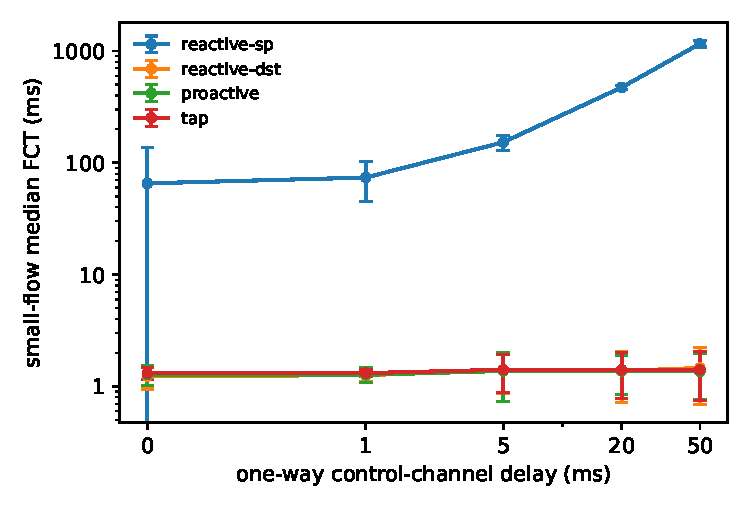
\includegraphics[width=\columnwidth]{ctrl_delay.pdf}
\caption{Small-flow median against one-way control-channel delay (university tree, mean of 3 seeds with 95\% intervals; log scales, the delay axis linear below 1\,ms). reactive-sp is exact-match reactive on shortest paths; reactive-dst is destination rules. Exact-match reactive's interval at 0\,ms extends below zero and is cut off.}\label{fig:delay}
\end{figure}

\textbf{In the median, only exact-match reactive pays for distance.} Its small-flow median rises by $+87$ [$+38$, $+137$]\,ms at 5\,ms, $+407$ [$+346$, $+468$]\,ms at 20\,ms and $+1{,}094$ [$+980$, $+1{,}208$]\,ms at 50\,ms; at 50\,ms the median is over one second in every seed. At 1\,ms the increase is not resolved ($+8$ [$-36$, $+53$]\,ms), because its median without delay already varies between seeds (47.5, 49.7 and 99.2\,ms). For destination rules, proactive and tap no change of the median is resolved at any delay; the intervals lie between $-0.52$ and $+0.87$\,ms. Destination rules do pay in the tail: at 50\,ms their small-flow mean rises by $+8.5$ [$+7.8$, $+9.2$]\,ms and their 99th percentile by $+355$ [$+243$, $+468$]\,ms, while no change in proactive's or tap's mean or 99th percentile is resolved.

\textbf{The slope is not explained.} From 20\,ms on, exact-match reactive's median grows by about 20--22\,ms per ms of one-way delay (20.3 at 20\,ms, 21.9 at 50\,ms), the equivalent of 10--11 control round trips per small flow. Its controller received 9.0--9.8 PACKET\_INs per flow at these delays. The logs count messages but do not record which of them lie on a flow's critical path, so we cannot attribute the slope, and we leave it unexplained.

Our delay is emulated on one machine and on one network; it is not a controller on a second PC.

\section{Where prediction has room: scale}\label{sec:scale}

The coarse-rule result depends on each pair carrying many flows while its rule is alive. At 54 hosts this no longer holds: the hit rate of pair rules falls to 50.8$\pm$5.0\% and of destination rules to 59.3$\pm$2.4\% (3 runs, about 640 flows over 2,862 pairs). Here the counter at a 10\% budget cannot be told apart from pair rules (51.1\%; paired difference $+0.3$ [$-2.4$, $+3.0$] points, 3 seeds) while using 1.9$\times$ their rules, and only the static oracle is clearly better (77.8\%; $+27.1$ [$+23.9$, $+30.2$]).

\textbf{A validated replay model.} To go beyond what the laptop can emulate we replay flow schedules through a timeout cache (idle 10\,s, hard 30\,s): a pair or destination rule is created on a miss at every switch of the path and refreshed by each packet of later flows. Replaying the stored schedules of all 46 measured pair- and destination-rule runs (four scenarios with 5 seeds, plus $k{=}6$ with 3) reproduces the measured hit rates with a mean absolute error per run of at most 0.1 percentage points in every scenario. We then generate web-search schedules with the same code for fat-trees with $k$ from 4 to 16 (16 to 1,024 hosts) at 5\% and 30\% load, 3 seeds each, and add a predictor that can actually be built: a frequency counter that pre-installs the busiest 10\% of pairs \emph{of the previous 30\,s window} (same pair popularity, new arrivals), with pair rules for everything else.

\begin{figure}[t]
\centering
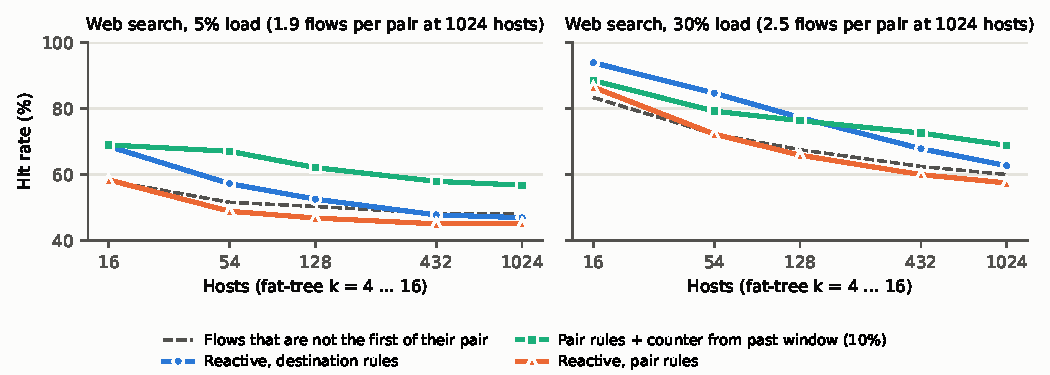
\includegraphics[width=\columnwidth]{scale_hit_rate.pdf}
\caption{Hit rate against network size (trace replay, web-search workload, mean of 3 seeds). The dash-dotted grey line is the share of flows that are not the first of their host pair.}\label{fig:scale}
\end{figure}

Figure~\ref{fig:scale} shows the result.
\begin{itemize}
\item \textbf{Coarse rules lose hit rate as flows per pair fall.} At 30\% load, destination rules fall from 93.9\% at 16 hosts to 62.6\% at 1,024; flows per active pair fall from 6.0 to 2.5. Pair rules track the share of flows that are not the first of their pair: their misses are almost all first flows, which no reactive rule can serve.
\item \textbf{At Zipf 1, prediction pays only in that regime.} At 16 hosts the history counter does not clearly beat destination rules: it trails by 5.4 points at 30\% load (88.5 vs.\ 93.9\%) and is within 0.4 points at 5\% (68.9 vs.\ 68.5\%, ahead in 2 of 3 seeds). At 30\% load it becomes the best non-hindsight strategy from 432 hosts (72.5 vs.\ 67.8\%; 68.8 vs.\ 62.6\% at 1,024). At 5\% load it beats destination rules by about 10 points from 54 hosts on.
\item \textbf{Hindsight references become uninformative at scale, and are not bounds.} A 10\% budget of all pairs exceeds the number of pairs that appear in a 30\,s window at 432 hosts and more (a 2\% budget does so at 5\% load), so an oracle that knows the future reaches 100\%; at 2\% and 30\% load it reaches 75.2\% at 432 hosts and 89.1\% at 1,024. Such references should be stated as a budget in rules, not as a share of pairs. They are also not upper bounds here: on top of pair rules, pre-installing a pair mainly saves its first miss, so the run's busiest pairs are not the best set, and the history counter beat the oracle in 4 of the 30 runs at a 2\% budget (by 0.1--1.7 points). Over longer runs the fixed oracle set also ages: with 120\,s of arrivals instead of 30\,s, oracle+10 falls by up to 15.9 points (Section~\ref{sec:discussion}).
\item \textbf{Skew matters as much as scale.} All of the above uses Zipf-1 pair popularity. Repeating the sweep with exponents 0, 0.5 and 1.5 (same sizes, loads and seeds) changes the picture. With weak or no skew (0, 0.5), flows per active pair are low (1.0--5.0) but the history counter never beats destination rules, at any size or load: it trails by 2.1--34.5 points, because the previous window says little about the next. With strong skew (1.5), flows per pair are high (4.7--29.7), and the counter beats destination rules in 9 of the 10 size/load cells by 1.6--6.6 points, at 16 hosts as well (88.0 vs.\ 81.7\% at 5\% load), where hit rates are already high. So flows per pair alone does not locate the regime: prediction needs pair popularity that is both skewed and stable, and its room on top of coarse rules shrinks as reuse grows. Our predictor sees a stationary ranking, which favours it.
\end{itemize}

The practical boundary is set by table size, not only by hit rate. Proactive forwarding with destination rules needs exactly one rule per host per switch: 1,024 rules per switch at 1,024 hosts, within the range of hardware tables of DevoFlow's era~\cite{devoflow}. Prediction therefore earns its keep in networks with more hosts than a switch can hold destination rules for, with skewed and stable pair popularity and few flows per pair: the case a predictor evaluation should target.

\section{Asking versus telling}\label{sec:tap}

A PACKET\_IN does two jobs: it \emph{asks} the controller where to send a packet, and it \emph{tells} the controller that a flow exists. Only asking delays the packet. Coarse rules and proactive installation remove the asking, but also the telling: with destination rules the controller hears of 0.4--6.4\% of connections on the small networks. Our tap controller keeps only the telling. Each switch has a destination rule per host, installed when it connects. At the switch a host is attached to, three higher-priority rules match TCP packets to that host with SYN (and not ACK), FIN or RST set; their actions forward the packet and send its first 128 bytes to the controller. No rule is installed per flow. TCP-flag matching is the Open vSwitch extension field \texttt{NXM\_NX\_TCP\_FLAGS}, sent from POX as a Nicira flow-mod; it is a standard match field in OpenFlow 1.5.

\begin{table}[t]
\caption{Tap against proactive and destination rules. Mean of 5 runs (3 at $k{=}6$); FCT is the small-flow median. Rules: largest peak over the runs, total (busiest switch). ``Heard'' is the share of connections the controller learns of.}\label{tab:tap}
\centering\footnotesize
\setlength{\tabcolsep}{2.6pt}
\begin{tabular}{@{}lrrrr@{}}
\toprule
Controller & FCT (ms) & PKT\_IN/s & Rules & Heard \\
\midrule
\multicolumn{5}{@{}l}{\emph{University tree, 16 hosts}} \\
Reactive, exact & 35.7$\pm$5.7 & 2,486 & 11,392 (3,654) & 100\% \\
Reactive, dest. & 0.9$\pm$0.4 & 3 & 80 (16) & 0.4\% \\
Proactive & 0.9$\pm$0.4 & 0 & 624 (192) & 0\% \\
Tap & 1.0$\pm$0.4 & 602 & 128 (28) & 100\% \\
\midrule
\multicolumn{5}{@{}l}{\emph{Abilene, 11 hosts}} \\
Reactive, exact & 57.8$\pm$2.2 & 452 & 5,430 (855) & 100\% \\
Reactive, dest. & 46.1$\pm$1.6 & 5 & 121 (11) & 2.2\% \\
Proactive & 46.0$\pm$1.5 & 0 & 386 (62) & 0\% \\
Tap & 46.1$\pm$1.5 & 174 & 154 (14) & 100\% \\
\midrule
\multicolumn{5}{@{}l}{\emph{Fat-tree $k{=}6$, web search 5\%, 54 hosts}} \\
Reactive, exact & 51.9$\pm$8.4 & 362 & 2,341 (160) & 100\% \\
Reactive, dest. & 12.7$\pm$4.0 & 154 & 804 (26) & 40.7\% \\
Proactive (ECMP) & 5.0$\pm$0.7 & 0 & 13,230 (312) & 0\% \\
Tap & 5.3$\pm$1.1 & 63 & 2,592 (63) & 100\% \\
\midrule
\multicolumn{5}{@{}l}{\emph{Fat-tree $k{=}4$, web search 30\%, 16 hosts}} \\
Reactive, dest. & 31.7$\pm$4.6 & 60 & 285 (16) & 6.4\% \\
Proactive (ECMP) & 29.6$\pm$5.5 & 0 & 1,072 (58) & 0\% \\
Tap & 39.3$\pm$21.9 & 109 & 368 (22) & 100\% \\
\bottomrule
\end{tabular}
\end{table}

\textbf{Speed and visibility together.} Table~\ref{tab:tap} is a separate batch from Table~\ref{tab:granularity}, run a month later, and its absolute times are not comparable with it (proactive on the campus tree: 0.94 against 1.49\,ms). Within the batch, on the university tree, Abilene and the 54-host fat-tree, tap's small-flow median is at most a fraction of a millisecond above proactive's: the paired differences are $+0.07$ [$-0.02$, $+0.15$], $+0.11$ [$-0.03$, $+0.24$] and $+0.33$ [$-0.18$, $+0.85$]\,ms (Table~\ref{tab:paired}). None of these is resolved, but tap was the slower of the two in 4 of 5, 4 of 5 and 3 of 3 seeds, and on Abilene its small-flow \emph{mean} is resolvably higher ($+0.12$ [$+0.01$, $+0.22$]\,ms). We therefore read the data as a small cost, bounded by the upper ends of these intervals, not as equal speed. The controller learned of all 46,641 connections in 18 runs, and again of all 46,641 in the 18 tap runs of the second batch (same seeds), with no switch errors. At 54 hosts, where coarse reactive rules miss often, tap's median is 2.4$\times$ lower than destination rules' and its controller receives 2.4$\times$ fewer messages (both differences resolved, in 3 of 3 seeds), while hearing of every connection rather than 41\%.

\textbf{Rules.} Tap needs fewer rules than pair-rule proactive (128 vs.\ 624; 2,592 vs.\ 13,230 at 54 hosts), but this saving is granularity, not tapping: proactive with destination rules needs $H\cdot S$ rules for $H$ hosts and $S$ switches (80 and 2,430), and tapping adds exactly $3H$ (48 and 162). The second batch measures this directly: tap minus proactive-dst is 48, 48, 33 and 162 rules on the four networks, $3H$ in each case.

\textbf{Cost.} About three copies per connection (602 PACKET\_IN/s and 14\% of one core at about 200 new connections per second on the university tree). No packet waits for the controller, but the copy rules are not free: against proactive-dst, which differs from tap only by them, tap's small-flow median is higher by $+0.08$ [$+0.05$, $+0.11$]\,ms on the campus tree and $+0.29$ [$+0.06$, $+0.51$]\,ms at 54 hosts (higher in every seed), with no measurable difference on Abilene ($-0.01$ [$-0.09$, $+0.07$]\,ms). We did not measure where in the switch this time goes.

\textbf{The $k{=}4$ fat-tree.} Here tap is slower than proactive ECMP (39.3 vs.\ 29.6\,ms) with a wide interval; one run had 3 failed flows of 1,111 and a 108\,ms mean, and large flows were slower in 4 of 5 runs. Tap spreads paths by destination, so all flows to one host share a path through the core, while proactive ECMP hashes per pair. To separate the copies from the paths we ran a second batch on the same laptop (same seeds, all four networks) that adds \emph{proactive-dst}: tap's destination rules on tap's paths, without the copy rules. On the $k{=}4$ fat-tree tap and proactive-dst have the same small-flow median within the batch (40.6 and 39.8\,ms; paired $+0.8$ [$-0.7$, $+2.3$]\,ms), against 30.0\,ms for proactive ECMP. The gap comes from one flow schedule: in seed 8 tap and proactive-dst fail the \emph{same} 7 flows and both have a 72.7--72.8\,ms median, while proactive ECMP has 23.9\,ms; in the other four seeds the three are mixed. Seed 8 was also the outlier of the first batch. So the slowdown belongs to destination-hashed paths, not to tapping. Because it rests on one seed, the paired difference proactive-dst $-$ proactive ECMP ($+9.8$ [$-17.6$, $+37.2$]\,ms) is not resolved.

\textbf{A frozen controller.} We stop the POX process for 5\,s, 10\,s into the university workload (3 seeds, about 1,000 connections per run start in the window). Under exact-match reactive, 3,029 of 3,030 such connections took over 1\,s (small-flow median 5.0--6.0\,s, the TCP SYN retransmission times). Under destination rules, proactive and tap, 4 did, all in one seed under all three controllers; tap's median in the window was 1.3--2.0\,ms against 1.2--1.7\,ms for proactive. Only tap still accounted for every connection (18,269 of 18,269): the copies queue while the controller is stopped and are read when it resumes.

\begin{table}[t]
\caption{Paired per-seed differences $A-B$ for the main claims: mean and 95\% interval (Student's $t$, $n{-}1$ df), and the number of seeds in which $A<B$. Hit rate in points, FCT (small-flow median) in ms. Bold: interval excludes zero. From \texttt{experiments/paired\_stats.py --paper}.}\label{tab:paired}
\centering\footnotesize
\setlength{\tabcolsep}{3pt}
\begin{tabular}{@{}llrrc@{}}
\toprule
$A - B$ & Metric & Mean & 95\% CI & $A{<}B$ \\
\midrule
\multicolumn{5}{@{}l}{\emph{Campus tree, 16 hosts ($n{=}5$; Tables~\ref{tab:granularity}, \ref{tab:tap})}} \\
Pair $-$ counter 25\% & hit & \textbf{+37.3} & [+30.7, +43.9] & 0/5 \\
Pair $-$ oracle 25\% & hit & \textbf{+29.8} & [+25.5, +34.1] & 0/5 \\
Dest. $-$ proactive & FCT & $-$0.02 & [$-$0.07, +0.03] & 4/5 \\
Tap $-$ proactive & FCT & +0.07 & [$-$0.02, +0.15] & 1/5 \\
\multicolumn{5}{@{}l}{\emph{Fat-tree $k{=}4$, 16 hosts ($n{=}5$)}} \\
Pair $-$ counter 25\% & hit & \textbf{+20.4} & [+18.7, +22.1] & 0/5 \\
Pair $-$ oracle 25\% & hit & \textbf{+12.4} & [+11.3, +13.6] & 0/5 \\
Dest. $-$ proactive ECMP & FCT & \textbf{+2.95} & [+0.01, +5.90] & 0/5 \\
Tap $-$ proactive ECMP & FCT & +9.6 & [$-$15.5, +34.7] & 2/5 \\
\multicolumn{5}{@{}l}{\emph{Abilene, 11 hosts ($n{=}5$)}} \\
Pair $-$ counter 25\% & hit & \textbf{+44.3} & [+42.5, +46.2] & 0/5 \\
Pair $-$ oracle 25\% & hit & \textbf{+37.3} & [+36.4, +38.2] & 0/5 \\
Dest. $-$ proactive & FCT & +0.06 & [$-$0.16, +0.27] & 2/5 \\
Tap $-$ proactive & FCT & +0.11 & [$-$0.03, +0.24] & 1/5 \\
\multicolumn{5}{@{}l}{\emph{Fat-tree $k{=}6$, 54 hosts ($n{=}3$)}} \\
Counter 10\% $-$ pair & hit & +0.3 & [$-$2.4, +3.0] & 1/3 \\
Oracle 10\% $-$ pair & hit & \textbf{+27.1} & [+23.9, +30.2] & 0/3 \\
Tap $-$ proactive ECMP & FCT & +0.33 & [$-$0.18, +0.85] & 0/3 \\
Tap $-$ dest. & FCT & \textbf{$-$7.38} & [$-$10.28, $-$4.47] & 3/3 \\
\multicolumn{5}{@{}l}{\emph{Second tap batch: proactive-dst = tap without copy rules}} \\
Tap $-$ p.-dst, tree & FCT & \textbf{+0.08} & [+0.05, +0.11] & 0/5 \\
Tap $-$ p.-dst, $k{=}4$ & FCT & +0.79 & [$-$0.69, +2.28] & 1/5 \\
Tap $-$ p.-dst, Abilene & FCT & $-$0.01 & [$-$0.09, +0.07] & 3/5 \\
Tap $-$ p.-dst, $k{=}6$ & FCT & \textbf{+0.29} & [+0.06, +0.51] & 0/3 \\
P.-dst $-$ proactive ECMP, $k{=}4$ & FCT & +9.80 & [$-$17.55, +37.15] & 3/5 \\
\bottomrule
\end{tabular}
\end{table}

\section{Discussion}\label{sec:discussion}

\textbf{For evaluations of rule predictors.} Our results suggest three requirements. (1) Compare against reactive with the same rule granularity as the pre-installed rules; otherwise the measured gain mixes coarseness and prediction. (2) Report flows per active pair (or per rule key) and the skew of pair popularity for the evaluated traffic; together they decide whether a coarse first-miss rule is reused and whether the past predicts the next pairs, and therefore whether prediction can add anything. (3) State hindsight bounds with a budget in rules and alongside a realisable predictor; at scale a share-of-pairs oracle is trivially perfect.

\textbf{When each strategy wins.} On small networks, or wherever a switch can hold one rule per destination, proactive destination rules are the smallest rule set that forwards all traffic without waiting, and on the campus tree, Abilene and the 54-host fat-tree they are as fast as pair-rule proactive within 0.1--0.5\,ms (paired: $+0.04$ [$-0.03$, $+0.10$], $-0.12$ [$-0.30$, $+0.07$], $-0.14$ [$-0.47$, $+0.19$]\,ms); on the $k{=}4$ fat-tree their destination-hashed paths lose one flow schedule badly. Coarse reactive rules come close. Exact-match reactive is justified only by per-flow policy, which our workloads do not exercise. In our model, prediction pays when pair popularity is skewed: at large scale for Zipf 1, by a few points at any size for Zipf 1.5, and not at all for near-uniform popularity. If the controller must know about each connection, tap provides that without the reactive wait, for TCP.

\textbf{Limitations.} The network is emulated in software, so there is no TCAM limit and no hardware rule-update rate; POX is single-threaded, so absolute controller numbers are POX's. The testbed networks have 11--54 hosts; larger sizes come from the replay model, which is validated for hit rate only, and its predictor is given stationary pair popularity, which favours prediction. Pair popularity is an assumed Zipf distribution except for the ISP workload, and the university size distribution was read from a published plot. Each run of Tables~\ref{tab:granularity} and~\ref{tab:tap} has 30\,s of arrivals, equal to the hard timeout, so on the testbed a rule installed on a first miss never reaches its hard timeout during the run. We checked the effect with the replay model (fat-trees $k{=}4$--8, both loads, 3 seeds): with 120\,s of arrivals, pair and destination rules gain 1.3--2.2 and 0.6--3.3 points of hit rate (more flows per pair outweigh the expiries), the history counter gains 1.4--9.4, and the static oracle at 10\% changes by $-15.9$ to $+1.3$. The comparisons that decide our conclusions do not change sign: destination rules stay 4.6--5.5 points ahead of the counter at 30\% load for $k{=}4$ and 6, and 9.6--16.4 points behind it at 5\% load for $k{=}6$ and 8 (means of 3 seeds, same sign in every seed). Two close cases move: at $k{=}8$, 30\% load, destination rules lead by 0.9 points at 30\,s and tie at 120\,s (79.19 vs.\ 79.19\%), and at $k{=}4$, 5\% load, the two are within one point at both lengths and swap order. So longer runs move the point where prediction starts to pay towards slightly smaller networks. On the testbed, 120\,s runs on the campus tree change pair and destination rules by at most 0.2 points and leave the counter 30 points below pair rules (Section~\ref{sec:hybrid}). Tap covers TCP only, records start and end but not bytes, and cannot take a decision before the first packet. The controller shares the host with the emulated network; a distant controller is emulated by delaying the OpenFlow channel on one network (Section~\ref{sec:delay}), not measured with a controller on a second machine, and the growth of exact-match reactive's delay with distance is not explained. Results come from batches on different days with the same settings; absolute times are compared only within a table.

\section{Conclusion}
In the pre-installation papers we surveyed, no predictor that pre-installs coarser rules is compared with a reactive baseline using the same coarse rules. When the reactive baseline uses the same coarse rules as the pre-installed ones, it reaches 86--100\% hit rates on networks of up to 16 hosts, above a budgeted popularity hybrid and its static oracle in every seed. In our validated replay model with Zipf-1 pair popularity, prediction becomes useful only when flows per host pair fall to 2--3: from 54 hosts at 5\% load and from about 432 hosts at 30\% load. It also needs skew: with near-uniform popularity it never helps, and with strong skew it adds a few points at every size. Separately, the visibility that reactive installation provides does not require making packets wait: copying connection start and end packets gives the controller every connection, at a small-flow median at most 0.2--0.9\,ms above proactive's on three of four networks. In the small-flow median, a distant controller costs only exact-match reactive: 50\,ms of one-way control-channel delay adds over a second to its small-flow median and less than 0.9\,ms to that of destination rules, proactive and tap. We release the benchmark so that future predictors can be measured against these baselines.

\balance
\begin{thebibliography}{99}
\bibitem{ethane} M. Casado, M.~J. Freedman, J. Pettit, J. Luo, N. McKeown, and S. Shenker, ``Ethane: Taking control of the enterprise,'' in \emph{Proc. ACM SIGCOMM}, 2007.
\bibitem{difane} M. Yu, J. Rexford, M.~J. Freedman, and J. Wang, ``Scalable flow-based networking with DIFANE,'' in \emph{Proc. ACM SIGCOMM}, 2010.
\bibitem{devoflow} A.~R. Curtis, J.~C. Mogul, J. Tourrilhes, P. Yalagandula, P. Sharma, and S. Banerjee, ``DevoFlow: Scaling flow management for high-performance networks,'' in \emph{Proc. ACM SIGCOMM}, 2011.
\bibitem{tootoonchian} A. Tootoonchian, S. Gorbunov, Y. Ganjali, M. Casado, and R. Sherwood, ``On controller performance in software-defined networks,'' in \emph{Proc. USENIX Hot-ICE}, 2012.
\bibitem{cacheflow} N. Katta, O. Alipourfard, J. Rexford, and D. Walker, ``CacheFlow: Dependency-aware rule-caching for software-defined networks,'' in \emph{Proc. ACM SOSR}, 2016.
\bibitem{smarttime} A. Vishnoi, R. Poddar, V. Mann, and S. Bhattacharya, ``Effective switch memory management in OpenFlow networks,'' in \emph{Proc. ACM DEBS}, 2014.
\bibitem{ahihta} B. Isyaku, K. Abu Bakar, M.~S. Mohd Zahid, and M.~N. Yusuf, ``Adaptive and hybrid idle--hard timeout allocation and flow eviction mechanism considering traffic characteristics,'' \emph{Electronics}, 2020.
\bibitem{pard} R. Rzepka, P. Boryło, A. Lasoń, and A. Szymański, ``PARD: Hybrid proactive and reactive method eliminating flow setup latency in SDN,'' \emph{J. Netw. Syst. Manag.}, vol.~28, 2020.
\bibitem{kim2022} Y. Kim, J. Park, and Y. Kyung, ``Mobility-aware hybrid flow rule cache scheme in software-defined access networks,'' \emph{Electronics}, vol.~11, no.~1, p.~160, 2022.
\bibitem{batista2024} Batista \emph{et al.}, ``A new intelligent scheduler to improve reactive OpenFlow communication in SDN-based IoT data streams,'' \emph{Discover Internet of Things}, vol.~4, no.~15, 2024.
\bibitem{rouf2025} A. Rouf and M. Yuksel, ``Spatial encoding of flow spaces for intelligent SDN applications,'' arXiv:2509.16485, 2025.

\bibitem{hariri2024} A. Hariri, M. Yuksel, and D. Mohaisen, ``RL-based speculative installation of unseen flows in SDNs for low-latency applications,'' in \emph{Proc. IEEE ICMLCN}, 2024, pp. 250--256.
\bibitem{metter2017} C. Metter, M. Seufert, F. Wamser, T. Zinner, and P. Tran-Gia, ``Analytical model for SDN signaling traffic and flow table occupancy and its application for various types of traffic,'' \emph{IEEE Trans. Netw. Serv. Manag.}, vol.~14, no.~3, 2017.
\bibitem{ipfix} B. Claise, B. Trammell, and P. Aitken, ``Specification of the IP Flow Information Export (IPFIX) protocol,'' RFC 7011, 2013.
\bibitem{everflow} Y. Zhu \emph{et al.}, ``Packet-level telemetry in large datacenter networks,'' in \emph{Proc. ACM SIGCOMM}, 2015.
\bibitem{flowsense} C. Yu, C. Lumezanu, Y. Zhang, V. Singh, G. Jiang, and H.~V. Madhyastha, ``FlowSense: Monitoring network utilization with zero measurement cost,'' in \emph{Proc. PAM}, 2013.
\bibitem{alfares} M. Al-Fares, A. Loukissas, and A. Vahdat, ``A scalable, commodity data center network architecture,'' in \emph{Proc. ACM SIGCOMM}, 2008.
\bibitem{hedera} M. Al-Fares, S. Radhakrishnan, B. Raghavan, N. Huang, and A. Vahdat, ``Hedera: Dynamic flow scheduling for data center networks,'' in \emph{Proc. USENIX NSDI}, 2010.
\bibitem{mininet} B. Lantz, B. Heller, and N. McKeown, ``A network in a laptop: Rapid prototyping for software-defined networks,'' in \emph{Proc. ACM HotNets}, 2010.
\bibitem{ovs} B. Pfaff \emph{et al.}, ``The design and implementation of Open vSwitch,'' in \emph{Proc. USENIX NSDI}, 2015.
\bibitem{benson} T. Benson, A. Akella, and D.~A. Maltz, ``Network traffic characteristics of data centers in the wild,'' in \emph{Proc. ACM IMC}, 2010.
\bibitem{dctcp} M. Alizadeh \emph{et al.}, ``Data center TCP (DCTCP),'' in \emph{Proc. ACM SIGCOMM}, 2010.
\bibitem{vl2} A. Greenberg \emph{et al.}, ``VL2: A scalable and flexible data center network,'' in \emph{Proc. ACM SIGCOMM}, 2009.
\bibitem{pfabric} M. Alizadeh \emph{et al.}, ``pFabric: Minimal near-optimal datacenter transport,'' in \emph{Proc. ACM SIGCOMM}, 2013.
\bibitem{pias} W. Bai, L. Chen, K. Chen, D. Han, C. Tian, and H. Wang, ``Information-agnostic flow scheduling for commodity data centers,'' in \emph{Proc. USENIX NSDI}, 2015.
\bibitem{zhang2005} Y. Zhang, Z. Ge, A. Greenberg, and M. Roughan, ``Network anomography,'' in \emph{Proc. ACM IMC}, 2005.
\bibitem{surge} P. Barford and M. Crovella, ``Generating representative web workloads for network and server performance evaluation,'' in \emph{Proc. ACM SIGMETRICS}, 1998.
\end{thebibliography}

\end{document}
